\documentclass[11pt,a4paper]{article}
\usepackage[utf8]{inputenc}
\usepackage[T1]{fontenc}
\usepackage[a4paper,margin=2.7cm]{geometry}
\usepackage{parskip}
\usepackage{enumitem}
\usepackage{titlesec}
\usepackage{xcolor}
\usepackage{booktabs}
\usepackage{array}
\usepackage{tikz}
\usepackage{graphicx}
\usepackage{pgfplots}
\pgfplotsset{compat=1.17}
\usepackage{needspace}

\titleformat{\section}{\large\bfseries}{\thesection}{0.5em}{}
\titleformat{\subsection}{\normalsize\bfseries}{\thesubsection}{0.5em}{}
\titlespacing*{\section}{0pt}{1.1cm}{0.4cm}
\titlespacing*{\subsection}{0pt}{0.7cm}{0.3cm}

\newcommand{\figcaption}[1]{\par\noindent\footnotesize\textbf{#1}\par\vspace{0.4cm}}

\begin{document}

\begin{titlepage}
\centering

\includegraphics[width=6cm]{img/fcefyn_logo.png}\\[1.0cm]

{\large Universidad Nacional de C\'ordoba}\\[0.1cm]
{\large Facultad de Ciencias Exactas, F\'isicas y Naturales}\\[2.0cm]

\rule{\linewidth}{0.5pt}\\[0.5cm]
{\LARGE\bfseries Monograf\'ia Final -- Avance}\\[0.4cm]
{\large Simulaci\'on y an\'alisis de congesti\'on en redes bajo distintos esquemas de encaminamiento}\\[0.5cm]
\rule{\linewidth}{0.5pt}\\[2.0cm]

{\large C\'atedra: Redes de Computadoras}\\[0.2cm]
{\large Docente: Santiago Mart\'in Henn}\\[1.5cm]

{\large\bfseries Grupo NetRunners}\\[0.6cm]
\begin{tabular}{c}
Bastida, Lucas Ramiro \\
Contessi, Rub\'en Andr\'es \\
Garay, Ignacio Hern\'an \\
Giraudo, Juan Pablo \\
Pe\~naloza, Gonzalo Adri\'an \\
Quinteros del Castillo, Tom\'as Agust\'in \\
Vasconsellos Blason, Benjam\'in Alejandro \\
\end{tabular}

\vfill
{\large 7 de noviembre de 2026}

\end{titlepage}

\section*{T\'itulo}

\noindent
Simulaci\'on y an\'alisis de congesti\'on en redes bajo distintos esquemas de encaminamiento

\section*{Introducci\'on}

\noindent
En una red de datos el tr\'afico nunca es parejo: depende de cu\'antos usuarios hay conectados en ese momento, qu\'e aplicaciones est\'an usando y hasta de la hora del d\'ia. Cuando ese tr\'afico crece demasiado y se acerca al l\'imite que pueden manejar los enlaces o los routers, aparece la congesti\'on, y ah\'i es cuando empiezan los problemas: paquetes que tardan m\'as de lo normal, p\'erdidas, descartes en los dispositivos intermedios.

Para este trabajo decidimos estudiar ese problema de forma pr\'actica. La idea es armar distintas topolog\'ias en GNS3, generar tr\'afico cada vez m\'as intenso entre los nodos y capturar todo con Wireshark para ver qu\'e va pasando a medida que la red se satura.

Nos interesan puntualmente dos cosas. Primero, qu\'e esquema de encaminamiento usa la red: no reacciona igual una red con rutas est\'aticas que una que corre RIP u OSPF cuando un camino empieza a saturarse. Segundo, qu\'e tipo de tr\'afico circula, porque tampoco es lo mismo TCP, que achica su ventana de transmisi\'on cuando detecta congesti\'on, que un flujo UDP en tiempo real, que sigue mandando datos sin importarle lo que est\'e pasando en la red.

La idea es ir desarrollando estos dos ejes a lo largo del trabajo y, sobre el final, comparar los resultados entre las distintas arquitecturas que simulemos, apoy\'andonos en los mecanismos de control de congesti\'on que vimos en la materia.

\section*{Objetivos}

\subsection*{Objetivo general}

\noindent
Analizar de forma experimental c\'omo se comportan distintas arquitecturas de red frente a condiciones de congesti\'on creciente, viendo qu\'e peso tienen el esquema de encaminamiento utilizado y los protocolos de capa de aplicaci\'on en el rendimiento final de la red.

\subsection*{Objetivos espec\'ificos}

\begin{itemize}[leftmargin=1.2cm]
  \item Armar en GNS3 al menos dos topolog\'ias con esquemas de encaminamiento distintos, para poder compararlas entre s\'i.
  \item Generar tr\'afico creciente entre los nodos de cada topolog\'ia hasta llegar a un punto de congesti\'on controlada.
  \item Usar Wireshark para capturar ese tr\'afico y revisar qu\'e indicadores de congesti\'on aparecen: p\'erdida de paquetes, mayor latencia, retransmisiones.
  \item Ver c\'omo responde el tr\'afico de distintos protocolos de aplicaci\'on ante la misma congesti\'on, por ejemplo HTTP sobre TCP frente a un flujo UDP en tiempo real.
  \item Relacionar lo que observemos en las capturas con los mecanismos de control de congesti\'on de TCP que dimos en clase (ventana de congesti\'on, arranque lento, retransmisi\'on r\'apida).
  \item Comparar el rendimiento de las arquitecturas simuladas seg\'un p\'erdida de paquetes, latencia y estabilidad del tr\'afico.
\end{itemize}

\section{Herramientas y entorno}
\label{sec:herramientas}

Antes de meternos con la parte experimental nos parece importante dejar documentado con qu\'e herramientas vamos a trabajar y por qu\'e, porque esto fue justo uno de los puntos que ajustamos despu\'es de la \'ultima devoluci\'on del profesor.

Vamos a armar las topolog\'ias en GNS3 en lugar de Packet Tracer. La diferencia clave es que GNS3 corre cada router y switch como una m\'aquina virtual real, con interfaces de red que s\'i existen a nivel del sistema operativo del host; Packet Tracer, en cambio, es un simulador cerrado donde el tr\'afico nunca sale de su propio motor interno. Packet Tracer trae su propio analizador de tr\'afico (el modo Simulaci\'on), pero, como se\~nal\'o el profesor, queda restringido al marco del simulador: no es el tr\'afico real de una placa de red. Como para nosotros es central poder capturar con Wireshark de verdad, GNS3 es la opci\'on que nos permite hacerlo sin ning\'un truco.

Para los routers vamos a usar la imagen de MikroTik CHR (\textit{Cloud Hosted Router}), que corre RouterOS, el mismo sistema operativo de los routers MikroTik f\'isicos. La elegimos por dos motivos: primero, porque MikroTik es una marca barata y muy com\'un en redes chicas en Argentina, as\'i que lo que configuremos ac\'a se traduce directamente a lo que configurar\'iamos en un equipo real (retomamos esto en la Secci\'on~\ref{sec:costos}); segundo, porque la licencia de prueba gratuita de CHR alcanza para todo lo que necesitamos, con la \'unica limitaci\'on de que capa la velocidad de cada interfaz a 1~Mbps, lo cual en realidad nos viene bien: nos da un cuello de botella ya armado sin tener que configurar \textit{traffic shaping} aparte (volvemos sobre esto en la Secci\'on~\ref{sec:metodologia}).

Wireshark se conecta directamente a los enlaces virtuales de GNS3: con el bot\'on derecho sobre cualquier cable de la topolog\'ia, la opci\'on ``Start capture'' abre una instancia de Wireshark escuchando esa interfaz virtual en tiempo real, igual que si fuera una placa de red f\'isica. Esto nos permite poner la captura justo en el punto de la red que nos interesa en cada corrida (por ejemplo, a la salida del nodo congestionado) sin necesidad de ning\'un adaptador externo.

Para generar el tr\'afico de prueba vamos a usar \texttt{iperf3} desde las puntas de la topolog\'ia (m\'aquinas Linux livianas dentro de GNS3), tanto en modo TCP como UDP; la Secci\'on~\ref{sec:metodologia} detalla c\'omo lo vamos a combinar con el cuello de botella para generar congesti\'on controlada.

\section{Marco te\'orico}

Esta secci\'on desarrolla los tres ejes que ya hab\'iamos adelantado en el plan de trabajo: control de congesti\'on (que es el centro de la monograf\'ia), encaminamiento y capa de aplicaci\'on. En cada uno tratamos de apoyarnos primero en lo que da Stallings, que es la bibliograf\'ia de la c\'atedra, y s\'olo recurrimos a otras fuentes cuando el libro no cubre algo con el detalle que necesitamos, como pasa con los protocolos de encaminamiento concretos y con algunos mecanismos de congesti\'on que quedaron desactualizados desde que se escribi\'o.

\subsection{Control de congesti\'on}
\label{sec:congestion}

La congesti\'on aparece cuando, en un nodo de la red (un conmutador, un router), el n\'umero de paquetes que llega empieza a acercarse al l\'imite de lo que ese nodo puede procesar y reenviar. Cada puerto de un nodo tiene colas de entrada y de salida, y si los paquetes llegan m\'as r\'apido de lo que se pueden transmitir, esas colas empiezan a crecer. Como ninguna memoria es infinita, tarde o temprano el nodo se queda sin lugar donde guardar paquetes nuevos y tiene que empezar a descartarlos (Stallings, Secci\'on 13.1).

Lo interesante es ver qu\'e pasa con el rendimiento de la red a medida que crece la carga. En un esquema ideal, el rendimiento crecer\'ia linealmente con la carga ofrecida hasta llegar a la capacidad m\'axima de la red, y a partir de ah\'i se mantendr\'ia constante. En la pr\'actica no pasa eso: como las memorias de los nodos son finitas, llega un punto en el que la red entra en una congesti\'on moderada (el rendimiento sigue creciendo pero cada vez m\'as despacio) y despu\'es en una congesti\'on severa, donde el rendimiento real empieza a caer aunque la carga siga aumentando. Esto pasa principalmente porque, cuando las colas se llenan, los nodos empiezan a descartar paquetes, los or\'igenes los retransmiten, y esa retransmisi\'on suma todav\'ia m\'as carga a una red que ya estaba saturada (Stallings, Secci\'on 13.1). El Gr\'afico~1 resume esta idea comparando el caso ideal con el real.

\needspace{1cm}
\begin{center}
\begin{minipage}{0.96\linewidth}
\centering
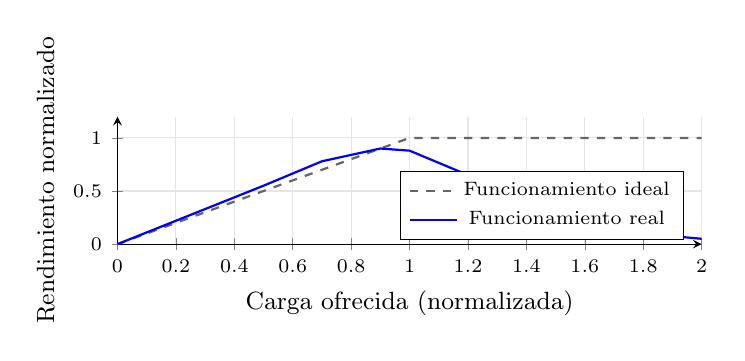
\begin{tikzpicture}
\begin{axis}[
  width=9cm, height=3.2cm,
  xlabel={Carga ofrecida (normalizada)},
  ylabel={Rendimiento normalizado},
  xmin=0, xmax=2, ymin=0, ymax=1.2,
  legend pos=south east,
  grid=major,
  grid style={gray!20},
  axis lines=left,
  label style={font=\small},
  tick label style={font=\scriptsize},
  legend style={font=\scriptsize},
]
\addplot[thick, dashed, color=black!60] coordinates {(0,0) (1,1) (2,1)};
\addlegendentry{Funcionamiento ideal}
\addplot[thick, color=blue] coordinates {(0,0) (0.5,0.55) (0.7,0.78) (0.9,0.9) (1.0,0.88) (1.2,0.65) (1.5,0.3) (1.8,0.1) (2,0.05)};
\addlegendentry{Funcionamiento real}
\end{axis}
\end{tikzpicture}
\figcaption{Gr\'afico 1. Rendimiento ideal vs. real de una red frente al aumento de la carga ofrecida (elaboraci\'on propia en base a Stallings, Figuras 13.3 y 13.4).}
\end{minipage}
\end{center}

Para evitar llegar a ese escenario, Stallings describe varios mecanismos de control de congesti\'on, cada uno pensado para intervenir en un punto distinto de la red. La contrapresi\'on act\'ua a nivel de enlace: el nodo congestionado frena a sus vecinos directos, y esa restricci\'on se va propagando hacia atr\'as hasta llegar al origen. Los paquetes de obstrucci\'on son m\'as directos: el nodo congestionado le manda al origen un paquete de control (el caso t\'ipico que da Stallings es el \textit{Source Quench} de ICMP) pidi\'endole que baje la velocidad de env\'io. Despu\'es est\'an las dos formas de se\~nalizaci\'on: la impl\'icita, que es la que usa TCP, donde el emisor infiere que hay congesti\'on por el aumento del retardo o por la p\'erdida de paquetes sin que la red le avise nada expl\'icitamente; y la expl\'icita, donde la red marca bits en los paquetes (hacia atr\'as o hacia adelante, como los bits BECN/FECN en retransmisi\'on de tramas) para notificarles a los extremos que hay congesti\'on en el camino (Stallings, Secci\'on 13.2).

Vale la pena una aclaraci\'on sobre estos dos \'ultimos mecanismos, porque quedaron un poco desactualizados desde que Stallings los describi\'o. El \textit{Source Quench} de ICMP est\'a formalmente deprecado desde el RFC~6633 (2013): en la pr\'actica, casi ning\'un sistema operativo moderno lo genera ni lo procesa, as\'i que si lo buscamos en nuestras capturas probablemente no lo vamos a encontrar. La se\~nalizaci\'on expl\'icita tampoco se qued\'o en BECN/FECN: su equivalente moderno en redes IP es ECN (\textit{Explicit Congestion Notification}, RFC~3168), que usa dos bits del encabezado IP para que un router marque un paquete en lugar de descartarlo cuando una cola empieza a llenarse, y el receptor le devuelve ese aviso al emisor para que reduzca la ventana sin necesidad de perder el paquete. Para que ECN tenga margen donde marcar en vez de descartar, adem\'as, conviene que los routers usen gesti\'on activa de colas, como RED (\textit{Random Early Detection}), en lugar del descarte de cola simple (\textit{tail drop}) que asumimos por defecto: RED empieza a descartar o marcar paquetes al azar un poco antes de que la cola se llene del todo, para avisar la congesti\'on de a poco en lugar de que se corten muchos flujos TCP al mismo tiempo.

Adem\'as de estos mecanismos, Stallings menciona la gesti\'on de tr\'afico como un conjunto de criterios adicionales para administrar la congesti\'on: la imparcialidad (que todos los flujos sufran la congesti\'on en una medida parecida, en vez de que un nodo descarte siempre los paquetes del mismo origen), la calidad de servicio (dar prioridad a los flujos m\'as sensibles al retardo, como voz o video, por sobre los que no lo son) y las reservas (acordar de antemano una velocidad de transmisi\'on, como hacen las redes ATM) (Stallings, Secci\'on 13.3). Esto nos va a servir m\'as adelante para justificar por qu\'e comparamos tr\'afico HTTP contra un flujo UDP en tiempo real: son dos tipos de tr\'afico con requisitos bien distintos frente a la congesti\'on (Stallings, Secci\'on 13.3).

\subsubsection*{La reacci\'on espec\'ifica de TCP}

Como una parte importante de nuestro tr\'afico simulado va a ser HTTP, que corre sobre TCP, nos interesa particularmente c\'omo reacciona TCP ante la congesti\'on. TCP no recibe ninguna se\~nal expl\'icita de la red: infiere que hay congesti\'on cuando detecta que un segmento se perdi\'o (porque expir\'o un temporizador de retransmisi\'on) o porque el retardo de ida y vuelta (RTT) empieza a crecer (Stallings, Secci\'on 20.3).

Para controlar cu\'anto puede enviar en cada momento, TCP usa una ventana de congesti\'on (\textit{cwnd}), que se suma al mecanismo de cr\'edito que ya conoc\'iamos de control de flujo. Cuando se abre una conexi\'on nueva, \textit{cwnd} arranca en un segmento y se duplica en cada tiempo de ida y vuelta mientras lleguen confirmaciones: esto es lo que se llama arranque lento, y hace que la ventana crezca exponencialmente al principio. Cuando \textit{cwnd} llega a un umbral (\textit{ssthresh}), TCP pasa a una fase m\'as conservadora, el ajuste din\'amico o evitaci\'on de congesti\'on, donde la ventana crece de a un segmento por cada tiempo de ida y vuelta en lugar de duplicarse. Si en alg\'un momento se pierde un segmento, TCP reduce el umbral a la mitad de la ventana actual, vuelve a poner \textit{cwnd} en uno y arranca todo el proceso de nuevo (Stallings, Secci\'on 20.3). El Gr\'afico~2 ilustra c\'omo se ve esta evoluci\'on a lo largo del tiempo.

\needspace{1cm}
\begin{center}
\begin{minipage}{0.96\linewidth}
\centering
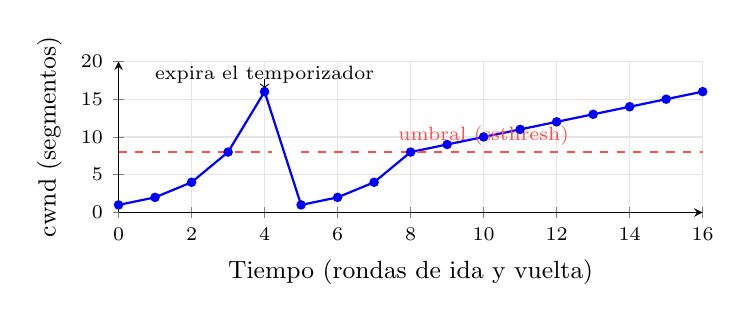
\begin{tikzpicture}
\begin{axis}[
  width=9cm, height=3.5cm,
  xlabel={Tiempo (rondas de ida y vuelta)},
  ylabel={cwnd (segmentos)},
  xmin=0, xmax=16, ymin=0, ymax=20,
  grid=major,
  grid style={gray!20},
  axis lines=left,
  label style={font=\small},
  tick label style={font=\scriptsize},
]
\addplot[thick, color=blue, mark=*, mark size=1.3pt] coordinates {
  (0,1) (1,2) (2,4) (3,8) (4,16) (5,1) (6,2) (7,4) (8,8) (9,9) (10,10) (11,11) (12,12) (13,13) (14,14) (15,15) (16,16)
};
\addplot[thick, dashed, color=red!70] coordinates {(0,8) (4.2,8)};
\addplot[thick, dashed, color=red!70] coordinates {(5,8) (16,8)};
\node[font=\scriptsize, color=red!70] at (axis cs: 10,10.2) {umbral (ssthresh)};
\node[font=\scriptsize] at (axis cs: 4,18.3) {expira el temporizador};
\draw[->, thin] (axis cs: 4,17.7) -- (axis cs: 4,16.4);
\end{axis}
\end{tikzpicture}
\figcaption{Gr\'afico 2. Evoluci\'on t\'ipica de la ventana de congesti\'on de TCP: arranque lento (crecimiento exponencial), ajuste din\'amico (crecimiento lineal) y ca\'ida ante una p\'erdida (elaboraci\'on propia en base a Stallings, Figura 20.13).}
\end{minipage}
\end{center}

Lo que describimos reci\'en es el comportamiento ante un \textit{timeout}: TCP asume lo peor y vuelve a arrancar desde \textit{cwnd} en uno. Pero hay otra forma de detectar la p\'erdida que no necesita esperar a que venza el temporizador: si el receptor sigue recibiendo segmentos fuera de orden, manda el mismo ACK repetido (ACK duplicado) por cada uno que llega; cuando el emisor ve tres ACKs duplicados seguidos, interpreta que un segmento se perdi\'o sin que haga falta esperar el \textit{timeout}, y lo retransmite de inmediato -- esto es la retransmisi\'on r\'apida. Como en este caso la red no necesariamente est\'a tan congestionada como en un \textit{timeout} (si siguen llegando segmentos post\'eriores, la red todav\'ia est\'a entregando paquetes), TCP no vuelve a arrancar de cero: reduce el umbral a la mitad y ajusta \textit{cwnd} a ese nuevo umbral en lugar de volver a uno, lo que se conoce como recuperaci\'on r\'apida. Esta diferencia es justamente uno de los indicadores que vamos a buscar en las capturas: una ca\'ida de \textit{cwnd} por ACKs duplicados deber\'ia verse distinta -- menos abrupta -- que una ca\'ida por \textit{timeout}.

Para decidir cu\'anto esperar antes de retransmitir un segmento, TCP necesita estimar el RTT. El algoritmo de Jacobson suaviza esa estimaci\'on combinando un promedio exponencial del RTT con una estimaci\'on de su variabilidad, en lugar de usar s\'olo un promedio simple, lo que lo hace mucho m\'as sensible a cambios bruscos en las condiciones de la red (Stallings, Secci\'on 20.3). El algoritmo de Karn, por su parte, resuelve un problema puntual: cuando un segmento se retransmite, no se puede saber con certeza si la confirmaci\'on que lleg\'o corresponde al env\'io original o a la retransmisi\'on, as\'i que esa muestra de RTT simplemente se descarta para no distorsionar la estimaci\'on (Stallings, Secci\'on 20.3). Estos dos mecanismos son los que vamos a buscar reflejados en las capturas de Wireshark cuando analicemos c\'omo reacciona TCP durante la simulaci\'on.

Una aclaraci\'on importante antes de pasar a las capturas: todo lo que describimos en esta secci\'on (arranque lento, ajuste din\'amico, ca\'ida a la mitad del umbral) corresponde a los algoritmos cl\'asicos que desarrolla Stallings, b\'asicamente Tahoe y Reno. El Linux que vamos a usar en las puntas de GNS3, sin embargo, usa CUBIC como algoritmo de control de congesti\'on por defecto desde hace ya varios a\~nos, que ajusta la ventana con una funci\'on c\'ubica del tiempo transcurrido desde la \'ultima p\'erdida en lugar del crecimiento lineal de Reno, pensada para aprovechar mejor enlaces de alta velocidad y alta latencia. Lo anticipamos ac\'a para no sorprendernos despu\'es: las capturas reales probablemente no van a calcar la forma exacta del Gr\'afico~2, aunque el patr\'on general -- crecimiento, ca\'ida ante p\'erdida, nuevo crecimiento -- se va a mantener.

\subsection{Encaminamiento}

El segundo eje tiene que ver con c\'omo decide la red por d\'onde mandar cada paquete, lo cual se vuelve clave cuando parte de la red empieza a congestionarse. Stallings presenta cuatro estrategias generales de encaminamiento, resumidas en la Tabla~1.

\needspace{1cm}
\begin{center}
\begin{minipage}{0.96\linewidth}
\centering
\scriptsize
\renewcommand{\arraystretch}{0.85}
\begin{tabular}{@{}p{2.3cm}p{5.2cm}p{3cm}p{3.2cm}@{}}
\toprule
\textbf{Estrategia} & \textbf{C\'omo decide la ruta} & \textbf{Ventaja principal} & \textbf{Desventaja principal} \\
\midrule
Est\'atica & Ruta fija precalculada para cada par origen-destino & Simplicidad, buen funcionamiento con carga estable & No reacciona ante fallos ni ante congesti\'on \\
Inundaci\'on & Cada nodo reenv\'ia por todos los enlaces salvo por el que lleg\'o el paquete & M\'axima robustez, asegura la entrega si existe alguna ruta & Genera una cantidad de tr\'afico muy alta \\
Aleatoria & El nodo elige al azar (o seg\'un una probabilidad) un enlace de salida & Sencilla, reparte la carga sin necesitar informaci\'on de la red & No sigue necesariamente la ruta de menor coste \\
Adaptable & Las decisiones cambian seg\'un el estado real de la red (fallos, congesti\'on) & Mejora el rendimiento percibido y ayuda a esquivar zonas congestionadas & M\'as compleja y puede generar oscilaciones si reacciona mal \\
\bottomrule
\end{tabular}
\par\vspace{0.1cm}
\figcaption{Tabla 1. Estrategias de encaminamiento (Stallings, Secci\'on 12.2).}
\end{minipage}
\end{center}

Dentro del encaminamiento adaptable, que es el que nos interesa porque es el que usan los protocolos din\'amicos como RIP y OSPF, Stallings desarrolla dos algoritmos de m\'inimo coste que son la base de casi todo el encaminamiento moderno. El algoritmo de Dijkstra necesita conocer la topolog\'ia completa de la red (todos los enlaces y sus costes) y va construyendo la ruta en etapas, incorporando en cada paso el nodo m\'as cercano que todav\'ia no forma parte del camino; es la base de OSPF. El de Bellman-Ford es m\'as austero: a cada nodo le alcanza con conocer el coste a sus vecinos directos, que va intercambiando peri\'odicamente con ellos en forma de vectores de distancia; es la base de RIP (Stallings, Secci\'on 12.3, p.~397--401).

Ac\'a es donde encontramos el l\'imite de Stallings para nuestro trabajo: el libro desarrolla los algoritmos de base, pero no entra en el detalle de los protocolos RIP, OSPF, EIGRP o BGP como tales. Como vamos a simular justamente RIP y OSPF en GNS3, para esta parte puntual recurrimos a Kurose y Ross, que s\'i los desarrolla en profundidad y es la referencia m\'as usada en la facultad como complemento de Stallings para esto. La Tabla~2 resume la comparaci\'on que vamos a usar como base para interpretar lo que veamos en las capturas.

\needspace{1cm}
\begin{center}
\begin{minipage}{0.96\linewidth}
\centering
\small
\begin{tabular}{@{}p{2.6cm}p{5.6cm}p{5.6cm}@{}}
\toprule
 & \textbf{RIP} & \textbf{OSPF} \\
\midrule
Algoritmo base & Bellman-Ford (vector distancia) & Dijkstra (estado de enlace) \\
M\'etrica & N\'umero de saltos (m\'aximo 15) & Costo configurable, t\'ipicamente en funci\'on del ancho de banda \\
Temporizadores & Actualizaci\'on 30~s, inv\'alido 180~s, purga 240~s & Hello 10~s, Dead 40~s \\
Transporte & UDP puerto 520, multicast 224.0.0.9 & IP directo, protocolo n\'umero 89 \\
Convergencia & M\'as lenta, puede sufrir el problema de ``cuenta a infinito'' & M\'as r\'apida ante cambios en la red \\
Escala t\'ipica & Redes peque\~nas o medianas & Redes grandes, organizadas en \'areas \\
\bottomrule
\end{tabular}
\par\vspace{0.1cm}
\figcaption{Tabla 2. RIP vs. OSPF (fuente: Kurose y Ross, \textit{Redes de Computadoras: un Enfoque Descendente}; RFC 2453 y RFC 2328).}
\end{minipage}
\end{center}

Para poder interpretar lo que capturemos con Wireshark, nos interesa bajar un escal\'on m\'as, de los algoritmos de base a c\'omo funcionan en concreto los protocolos que vamos a simular.

RIPv2 (RFC~2453) manda su tabla completa de rutas cada 30~segundos por multicast (224.0.0.9) sobre UDP, puerto 520. Si un router deja de recibir actualizaciones de un vecino durante 180~segundos, marca esa ruta como inv\'alida, y a los 240~segundos (sin que haya llegado una actualizaci\'on que la corrija) la purga definitivamente de la tabla; estos tres tiempos son justamente los que explican por qu\'e RIP tarda tanto en darse cuenta de que algo cambi\'o. Para evitar el problema cl\'asico de ``cuenta a infinito'' (dos routers pas\'andose entre s\'i una ruta ca\'ida como si todav\'ia existiera), RIP combina horizonte dividido (no anunciarle a un vecino una ruta que se aprendi\'o de \'el mismo) con envenenamiento en reversa (anunciar esa ruta de vuelta, pero con m\'etrica infinita, en lugar de simplemente omitirla) y \textit{hold-down} (ignorar por un tiempo cualquier anuncio que empeore una ruta reci\'en ca\'ida, por si es informaci\'on vieja que todav\'ia est\'a circulando). Las actualizaciones disparadas (mandar la tabla apenas cambia algo, sin esperar los 30~segundos) ayudan a que la convergencia no dependa \'unicamente del temporizador peri\'odico.

OSPF (RFC~2328) funciona distinto: en lugar de mandar toda la tabla peri\'odicamente, cada router arma una base de datos de estado de enlace (LSDB) a partir de anuncios (LSA, de distintos tipos seg\'un qu\'e describan) que intercambia y sincroniza con sus vecinos solo cuando algo cambia. Los vecinos se descubren y se mantienen con paquetes Hello cada 10~segundos; si un vecino no manda un Hello en 40~segundos (el temporizador \textit{Dead}), se lo da de baja y se recalcula. En redes multiacceso (como una LAN con varios routers), OSPF elige un router designado (DR) y uno de respaldo (BDR) para que los dem\'as sincronicen la LSDB solo con ellos y no entre todos contra todos, y para que la red no crezca indefinidamente en una sola LSDB permite dividirla en \'areas, donde el \'area~0 (\textit{backbone}) conecta a todas las dem\'as. OSPF corre directamente sobre IP, con el protocolo n\'umero 89, sin pasar por UDP ni TCP.

La m\'etrica de OSPF merece una aclaraci\'on aparte, porque nos puede jugar en contra si no la ajustamos: el costo de un enlace se calcula como un ancho de banda de referencia dividido el ancho de banda real del enlace, y por defecto, en equipos Cisco, esa referencia es 100~Mbps. El problema es que, si no tocamos ese valor con \texttt{auto-cost reference-bandwidth}, cualquier enlace de 100~Mbps o m\'as nos queda con costo~1, as\'i que OSPF termina sin poder distinguir un enlace de 100~Mbps de uno de 1~Gbps y elige caminos casi como si solo contara saltos. Como en nuestras topolog\'ias vamos a tener un enlace deliberadamente angosto (el cuello de botella que armamos a prop\'osito, Secci\'on~\ref{sec:metodologia}), vamos a tener que revisar este valor para que el costo realmente refleje esa diferencia.

Para completar el panorama de las rutas est\'aticas que ya mencionamos en la Tabla~1: cada ruta, est\'atica o aprendida por un protocolo, tiene asociada una distancia administrativa, que es lo que un router usa para decidir cu\'al preferir cuando aprende la misma ruta por m\'as de una fuente (cuanto m\'as baja, m\'as confiable se la considera; una ruta est\'atica suele tener distancia administrativa~1, m\'as confiable que RIP~120 u OSPF~110). Esto permite armar rutas est\'aticas flotantes: una ruta est\'atica con distancia administrativa deliberadamente alta, que el router ignora mientras tenga una ruta mejor (por ejemplo, aprendida por OSPF) y que solo entra en uso si esa ruta mejor desaparece -- una forma de darle a la red est\'atica algo de respaldo ante una ca\'ida sin volverla din\'amica.

\subsubsection*{El punto clave para nuestro tema}

Ac\'a aparece algo que nos parece central para el experimento: ni RIP ni OSPF reaccionan a la congesti\'on. Sus m\'etricas son fijas -- RIP cuenta saltos, OSPF usa el ancho de banda nominal del enlace -- y ninguna de las dos depende de cu\'anta carga real est\'a circulando en ese momento. Esto significa que, si satur\'amos un enlace sin tirarlo abajo, ni RIP ni OSPF van a cambiar de ruta: van a seguir mandando tr\'afico por el mismo camino saturado, porque desde su punto de vista el enlace sigue arriba y con el mismo costo que antes. Esto cambia lo que podemos esperar de la comparaci\'on: la diferencia entre est\'atica, RIP y OSPF que vamos a poder mostrar no es ``cu\'al evita mejor la congesti\'on'', sino m\'as bien c\'omo converge cada una ante una falla y qu\'e tan r\'apido.

Para que esta comparaci\'on no se quede solo en eso, nos parece importante contrastarla con tres ideas m\'as:

\begin{itemize}
  \item \textbf{ECMP} (\textit{Equal-Cost Multi-Path}): tanto RIP como OSPF pueden repartir tr\'afico entre varios caminos si tienen el mismo costo. Si dise\~namos alguna de nuestras topolog\'ias con dos caminos equivalentes entre origen y destino, ah\'i s\'i podr\'iamos ver una diferencia real de rendimiento contra la est\'atica, que normalmente usa un solo camino fijo.
  \item \textbf{EIGRP} (protocolo propietario de Cisco, sin RFC asociado): a diferencia de RIP y OSPF, su m\'etrica compuesta puede incluir la carga del enlace (uno de los llamados pesos~K), aunque viene desactivada por defecto. Mencionarlo sirve para explicar por qu\'e, en la pr\'actica, casi nadie rutea seg\'un la carga: el riesgo son las oscilaciones de rutas que ya aparecen como desventaja del encaminamiento adaptable en la Tabla~1 (una ruta se descongestiona, el tr\'afico vuelve a ella, se vuelve a congestionar, y as\'i).
  \item \textbf{Ingenier\'ia de tr\'afico} (MPLS-TE, SD-WAN): es la soluci\'on que s\'i se usa en redes reales para este problema -- elegir caminos seg\'un la carga real, no solo seg\'un un costo fijo --, aunque queda fuera del alcance de nuestra simulaci\'on. La mencionamos solo como contexto de hacia d\'onde apunta la industria.
\end{itemize}

BGP, por su parte, tambi\'en queda fuera del alcance directo de nuestra simulaci\'on, pero lo mencionamos porque es el protocolo que efectivamente usa Internet para el encaminamiento entre sistemas aut\'onomos, definido en el RFC~4271; a diferencia de RIP y OSPF, que rutean dentro de una misma organizaci\'on, BGP decide c\'omo se conectan organizaciones distintas entre s\'i.

\subsection{Capa de aplicaci\'on}
\label{sec:aplicacion}

El tercer eje tiene que ver con qu\'e protocolos de aplicaci\'on vamos a usar para generar el tr\'afico que despu\'es vamos a congestionar. Nos centramos en tres, porque se complementan bien para nuestro objetivo de comparar tr\'afico reactivo a la congesti\'on contra tr\'afico que no lo es.

HTTP es el protocolo que vamos a usar para generar el tr\'afico principal de la simulaci\'on. Corre sobre TCP, y ac\'a conviene ser precisos con la versi\'on: en HTTP/1.0 cada solicitud abr\'ia y cerraba su propia conexi\'on TCP, as\'i que una p\'agina con varios recursos implicaba repetir todo el mecanismo de apertura de conexi\'on -- y con \'el, todo el arranque lento de TCP que desarrollamos en la Secci\'on~\ref{sec:congestion} -- una y otra vez. HTTP/1.1, que es la versi\'on que vamos a usar como base, soluciona esto con conexiones persistentes: una misma conexi\'on TCP se reutiliza para varias solicitudes seguidas, lo que evita pagar el arranque lento en cada una (Stallings, Secci\'on 22.2). Versiones m\'as nuevas van todav\'ia m\'as lejos: HTTP/2 multiplexa varias solicitudes en paralelo sobre una \'unica conexi\'on TCP, y HTTP/3 directamente deja TCP y corre sobre QUIC, que viaja sobre UDP pero implementa su propio control de congesti\'on a nivel de aplicaci\'on en lugar de depender del de TCP. Para nuestro trabajo esto importa porque, al usar HTTP/1.1 sobre TCP cl\'asico, el tr\'afico que generemos s\'i va a mostrar los efectos del arranque lento y de la reducci\'on de la ventana ante la congesti\'on -- que es justamente lo que nos interesa observar --, algo que con HTTP/3 ser\'ia mucho menos directo de interpretar.

El segundo protocolo que nos interesa desarrollar es RTP (\textit{Real-time Transport Protocol}) sobre UDP, porque es el contraste real que nos faltaba frente a HTTP: en los objetivos planteamos comparar tr\'afico reactivo a la congesti\'on contra un flujo UDP en tiempo real, y hasta ahora solo hab\'iamos desarrollado SNMP, que no sirve para eso porque es tr\'afico de gesti\'on, no de usuario. RTP es el protocolo que usan las aplicaciones de voz y video (una videollamada, streaming en vivo) para empaquetar audio y video sobre UDP, con n\'umero de secuencia y marca de tiempo para que el receptor pueda reordenar y reproducir a un ritmo constante. La diferencia clave con TCP/HTTP es que RTP no retransmite: si se pierde un paquete de audio de hace medio segundo, retransmitirlo no sirve de nada porque para cuando llegue ya pas\'o el momento de reproducirlo, as\'i que el receptor simplemente lo salta y sigue. Lo que s\'i le importa a este tipo de tr\'afico es el \textit{jitter} (la variaci\'on en el tiempo de llegada entre paquetes consecutivos), porque si var\'ia demasiado el buffer de reproducci\'on se queda sin datos o se desborda; y tolera cierta p\'erdida de paquetes, hasta un punto, sin que la calidad percibida se caiga demasiado. Esto es exactamente lo opuesto a c\'omo reacciona TCP, y es lo que vamos a poder contrastar generando un flujo RTP simulado -- por ejemplo con \texttt{iperf3} en modo UDP a tasa fija -- en paralelo con el tr\'afico HTTP.

SNMP, por su parte, lo traemos a colaci\'on por un motivo distinto. Es el protocolo est\'andar para la gesti\'on de redes: una estaci\'on de gesti\'on consulta o modifica variables (objetos MIB) de los agentes instalados en los dispositivos de la red mediante mensajes \texttt{Get}, \texttt{Set} y notificaciones as\'incronas (\textit{traps}) (Stallings, Secci\'on 22.3). A diferencia de HTTP, SNMP corre sobre UDP, as\'i que no hereda ning\'un mecanismo de control de congesti\'on: si se pierde un mensaje, simplemente se pierde. Nos interesa mencionarlo porque, en una red real, SNMP ser\'ia justamente la herramienta que se usar\'ia para monitorear de forma autom\'atica los mismos indicadores de congesti\'on que nosotros vamos a observar ``a mano'' con Wireshark (p\'erdida de paquetes, uso de los enlaces), lo que nos permite conectar nuestra simulaci\'on con c\'omo se manejar\'ia este mismo problema en producci\'on.

En conjunto, estos tres ejes nos dan el marco que necesit\'abamos para dise\~nar la parte experimental: sabemos qu\'e mecanismos de congesti\'on vamos a buscar en las capturas, qu\'e protocolos de encaminamiento vamos a comparar y qu\'e tipo de tr\'afico vamos a generar para poner a prueba todo esto.

\section{Metodolog\'ia}
\label{sec:metodologia}

Esta secci\'on describe c\'omo vamos a generar la congesti\'on, qu\'e vamos a medir y con qu\'e herramienta, y c\'omo vamos a estructurar el an\'alisis de los resultados -- este \'ultimo punto fue justamente lo que nos pidi\'o reforzar el profesor en su devoluci\'on.

\subsection*{El cuello de botella}

Antes de simular nada nos topamos con un problema pr\'actico: en GNS3, por defecto, los enlaces virtuales no tienen ning\'un l\'imite real de ancho de banda, as\'i que si no configuramos nada, nunca vamos a lograr congestionar la red por m\'as tr\'afico que generemos. Como ya mencionamos en la Secci\'on~\ref{sec:herramientas}, la licencia gratuita de MikroTik CHR limita cada interfaz a 1~Mbps, lo cual nos resuelve el problema casi de arranque: ese l\'imite va a actuar como el cuello de botella de la topolog\'ia. Donde haga falta un control m\'as fino -- por ejemplo, para que el cuello de botella quede en un punto espec\'ifico de la red y no en todas las interfaces por igual -- lo vamos a complementar con colas configuradas en el router o con \texttt{tc} (\textit{traffic control}) directamente en las puntas Linux.

\subsection*{Generaci\'on de tr\'afico y m\'etricas}

Para generar tr\'afico de prueba entre las puntas de la topolog\'ia vamos a usar \texttt{iperf3}, que nos permite tanto tr\'afico TCP (para ver el comportamiento de HTTP) como UDP a tasa fija (para simular el flujo RTP en tiempo real que describimos en la Secci\'on~\ref{sec:aplicacion}). La Tabla~3 resume qu\'e herramienta usamos para medir cada m\'etrica.

\needspace{1cm}
\begin{center}
\begin{minipage}{0.96\linewidth}
\centering
\small
\begin{tabular}{@{}p{4.3cm}p{9.3cm}@{}}
\toprule
\textbf{M\'etrica} & \textbf{Herramienta} \\
\midrule
Throughput TCP & \texttt{iperf3} en modo TCP + I/O Graphs de Wireshark \\
Throughput, jitter y p\'erdida UDP & \texttt{iperf3} en modo UDP con tasa fija (\texttt{-b}) \\
Latencia & \texttt{ping} (RTT) \\
Arranque lento y ca\'ida de \textit{cwnd} & Wireshark, Statistics~$\to$~TCP Stream Graphs (gr\'afico de Stevens / \textit{tcptrace}) \\
Tiempo de convergencia & Cortar un enlace y medir cu\'anto tardan en volver los \texttt{ping}s, capturando los paquetes de RIP/OSPF \\
\bottomrule
\end{tabular}
\par\vspace{0.1cm}
\figcaption{Tabla 3. M\'etricas a registrar y herramienta usada para cada una.}
\end{minipage}
\end{center}

\subsection*{De detectar a explicar}

El profesor nos marc\'o algo importante en la devoluci\'on: no alcanza con mostrar que hay una diferencia entre las capturas de las distintas topolog\'ias, hay que explicarla. Para que esto no quede librado a c\'omo le salga a cada uno, proponemos que cada resultado que presentemos siga siempre la misma estructura de tres pasos: primero, qu\'e observamos concretamente en la captura (el n\'umero, el gr\'afico, el paquete puntual); segundo, qu\'e predec\'ia la teor\'ia que desarrollamos en el marco te\'orico, con referencia expl\'icita a la secci\'on correspondiente; y tercero, por qu\'e coincide o por qu\'e no -- y si no coincide, qu\'e variable de nuestra simulaci\'on (por ejemplo, que usamos CUBIC en lugar de Reno, o que no ajustamos el costo de referencia de OSPF) puede explicar la diferencia.

\subsection*{Cronograma}

Con la semana extra que nos dio el profesor, as\'i pensamos seguir hasta el 9 de noviembre:

\begin{itemize}
  \item Primero vamos a armar las topolog\'ias en GNS3: al menos dos id\'enticas entre s\'i, que solo se diferencien en el esquema de encaminamiento (est\'atica y RIP seguro, OSPF si llegamos con los tiempos), dejando documentado c\'omo generamos el tr\'afico creciente y qu\'e m\'etricas anotamos en cada corrida.
  \item Con eso armado, corremos las capturas con Wireshark en los mismos puntos de cada topolog\'ia para que las corridas sean realmente comparables entre s\'i.
  \item Despu\'es viene lo m\'as laborioso: cruzar lo que vimos en las capturas con lo que desarrollamos ac\'a, siguiendo la estructura de tres pasos que planteamos arriba (por ejemplo, encontrar en una captura real el arranque lento de TCP que graficamos, o ver si RIP tarda m\'as en converger que OSPF como dice la teor\'ia, y explicar por qu\'e).
  \item En paralelo, cerramos la secci\'on de implementaci\'on real y costos (Secci\'on~\ref{sec:costos}) con las cotizaciones definitivas.
  \item Y cerramos con las conclusiones, volviendo a los objetivos que planteamos al principio para ver qu\'e tanto los cumplimos, sin esconder las limitaciones de trabajar con una simulaci\'on y no con una red real.
\end{itemize}

\section{Implementaci\'on real y costos}
\label{sec:costos}

Esta secci\'on responde al \'ultimo pedido del profesor: ponerle nombre, apellido y precio a los equipos, distinguiendo entre lo que usamos gratis para simular en la facultad y lo que costar\'ia armar esto mismo con hardware real.

\subsection*{Alcance: nuestra propia topolog\'ia, no una red hipot\'etica de empresa}

En vez de inventar un escenario de red que no se corresponde con lo que realmente vamos a simular, decidimos cotizar lo que har\'ia falta para armar nuestra propia topolog\'ia de laboratorio con equipos f\'isicos: dos routers (conectados entre s\'i por el enlace que usamos como cuello de botella), dos switches (uno de cada lado, para conectar las puntas) y dos computadoras o servidores livianos que hacen de cliente y servidor de \texttt{iperf3}. Es el mismo hardware para las tres variantes de encaminamiento que comparamos (est\'atica, RIP, OSPF): en la pr\'actica no har\'ia falta comprarlo tres veces, alcanzar\'ia con reconfigurar los mismos equipos entre corrida y corrida, as\'i que cotizamos un solo juego.

\subsection*{Simulaci\'on en GNS3: costo \$0}

Todo lo que usamos en la computadora para simular es gratuito o de c\'odigo abierto: GNS3, Wireshark e iperf3/Linux no tienen costo de licencia, y la imagen de router que elegimos, MikroTik CHR, tiene una versi\'on de prueba gratuita que alcanza para simular todas las funciones de ruteo que necesitamos (la \'unica limitaci\'on es que capa la velocidad a 1~Mbps por interfaz, que como ya dijimos nos viene bien como cuello de botella). Esto es justamente parte de lo que nos interesa remarcar: la simulaci\'on no cuesta nada, pero no refleja el costo de montar la red de verdad.

\subsection*{Equipos reales: tres niveles de calidad}

Para la implementaci\'on real armamos tres opciones por rol, pensando en el tri\'angulo calidad / tiempo / presupuesto que nos pidi\'o el profesor. Los precios son los que cotiz\'o uno de nuestros compa\~neros en el mercado argentino; los convertimos a pesos con el tipo de cambio oficial del 28 de octubre de 2026 (\$1.560 por d\'olar, fuente: indicadores.ar) para que el n\'umero final tenga sentido en nuestro contexto, ya que un precio en d\'olares sin fecha ni tipo de cambio no dice mucho en la Argentina de hoy.

\needspace{1cm}
\begin{center}
\begin{minipage}{0.96\linewidth}
\centering
\small
\begin{tabular}{@{}p{2.3cm}p{3.65cm}p{3.65cm}p{3.65cm}@{}}
\toprule
\textbf{Rol} & \textbf{Econ\'omico} & \textbf{Intermedio} & \textbf{Empresarial} \\
\midrule
Router de n\'ucleo / borde & MikroTik hEX~S o RB750Gr3 (USD 70--120) & Cisco Router serie 900 / Ubiquiti UniFi Gateway (USD 300--600) & Cisco ISR~1100 / Catalyst~8000 (USD 1.500--3.500+, m\'as licencias IOS~XE) \\
Switch & MikroTik CSS326 / TP-Link Smart Managed (USD 100--180) & Cisco Business 250/350 Series (USD 300--500) & Cisco Catalyst 9200/9300 (USD 1.800--4.000+) \\
Monitoreo (SNMP) & Zabbix / LibreNMS, software libre (USD 0) & Zabbix / LibreNMS (USD 0) & PRTG Network Monitor (desde USD 1.800) \\
\bottomrule
\end{tabular}
\par\vspace{0.1cm}
\figcaption{Tabla 4. Equipos por rol y nivel de calidad, para armar nuestra propia topolog\'ia de laboratorio con hardware real.}
\end{minipage}
\end{center}

\needspace{1cm}
\begin{center}
\begin{minipage}{0.96\linewidth}
\centering
\small
\begin{tabular}{@{}p{3.6cm}p{4.2cm}p{4.2cm}@{}}
\toprule
\textbf{Nivel} & \textbf{Total aprox. (USD)} & \textbf{Total aprox. (ARS, \$1.560/USD)} \\
\midrule
Econ\'omico & USD 200--350 & \$312.000 -- \$546.000 \\
Intermedio & USD 700--1.200 & \$1.092.000 -- \$1.872.000 \\
Empresarial & USD 5.000+ & \$7.800.000+ \\
\bottomrule
\end{tabular}
\par\vspace{0.1cm}
\figcaption{Tabla 5. Costo total aproximado por nivel, cotizado por el grupo en el mercado argentino (28/10/2026, d\'olar oficial \$1.560 -- fuente: indicadores.ar).}
\end{minipage}
\end{center}

\subsection*{Que lo emulado coincida con lo que se compra}

No es casualidad que hayamos elegido MikroTik CHR para emular los routers: corre RouterOS, el mismo sistema operativo que traen los routers MikroTik f\'isicos, as\'i que la configuraci\'on que armamos en GNS3 (rutas est\'aticas, RIP, OSPF) es literalmente la misma que usar\'iamos en el equipo real de nivel econ\'omico. Si hubi\'eramos elegido Cisco IOSv, en cambio, hubi\'eramos necesitado una licencia paga (CML) para emularlo, y los equipos Cisco reales son m\'as caros e incluyen contratos de soporte -- lo cual tiene sentido para el nivel empresarial, pero no para validar nuestra topolog\'ia de laboratorio.

\subsection*{Monitoreo}

Ya mencionamos SNMP en la Secci\'on~\ref{sec:aplicacion} como el protocolo que se usar\'ia en producci\'on para monitorear autom\'aticamente los mismos indicadores que nosotros observamos ``a mano'' con Wireshark. Ac\'a tambi\'en hay una decisi\'on de costo: herramientas de monitoreo libres como Zabbix o LibreNMS no tienen costo de licencia y alcanzan perfectamente para una red de nuestro tama\~no, mientras que una herramienta paga como PRTG Network Monitor (desde aproximadamente USD~1.800 de licencia) suma funcionalidades pensadas para redes mucho m\'as grandes, que para nuestro caso ser\'ian un gasto innecesario.

\subsection*{Calidad, tiempo y presupuesto}

Cerramos con c\'omo pensamos el triple borde que nos pidi\'o el profesor, aplicado a nuestro propio caso:

\begin{itemize}
  \item La \textbf{ruta est\'atica} es la opci\'on m\'as barata en equipos -- no necesita routers con soporte de protocolos din\'amicos avanzados -- pero la m\'as cara en horas de operaci\'on: cada cambio en la red hay que cargarlo a mano, y un error humano tarda en notarse.
  \item \textbf{OSPF} necesita personal m\'as capacitado para configurarlo y mantenerlo bien (\'areas, costos, autenticaci\'on), pero una vez armado escala mejor y converge mucho m\'as r\'apido que RIP ante una ca\'ida.
  \item Para nuestro propio escenario de laboratorio, el nivel econ\'omico (USD~200--350) ya alcanza para validar todo lo que planteamos: los tres esquemas de encaminamiento, el cuello de botella y las capturas. El nivel intermedio (USD~700--1.200) tendr\'ia sentido reci\'en si pensamos en una red que vaya a seguir creciendo despu\'es del laboratorio; el nivel empresarial (USD~5.000+) queda totalmente fuera de escala para lo que necesitamos nosotros, pero lo dejamos documentado porque muestra hasta d\'onde llega el mismo problema de encaminamiento cuando la red es mucho m\'as grande.
\end{itemize}

\section*{Estado actual}

Con estos cambios creemos que respondimos a todo lo que marc\'o el profesor en su \'ultima devoluci\'on: ampliamos el marco te\'orico de encaminamiento y capa de aplicaci\'on, dejamos la metodolog\'ia apuntada a explicar y no solo detectar, y sumamos la secci\'on de implementaci\'on real y costos. Nos encantar\'ia que le vuelva a pegar una mirada antes de que nos pongamos a armar las topolog\'ias en GNS3, por si queda algo para ajustar.

\end{document}
